\chapter{Implementation Details}
\label{ch:implementation}

\section{Chapter Overview}

In this chapter, the discussion will be about the technical design of the various functional modules starting with the Authentication Module. This program creates a secured environment where access controls are implemented based on Role-Based Access Control (RBAC). The Students  Applicants Module is designed for the creation of profiles, handling multi-form applications, and automatic PDF file creation. Lastly, the Administration Module will act as the main module which facilitates all the data-related functions as well as monitoring functions in the system.

\noindent Other areas included in the development of this implementation will be special workflow designs for Dean, Registrar, Hall, and Medical modules. Through these modules, applicants can be verified, and all the required data can be validated prior to making the admission official. At last, we will discuss in this chapter the process for System Integration, focusing on integration with cloud storage and other third-party systems.

\section{Introduction}

This chapter discusses the detailed implementation aspects of the Digital Admission Procedure Management for Post-GST Candidates (JUST-DAPM-PGC). It presents the actual user interfaces developed, focusing on the workflows, data handling, and specific functionalities of different user roles, starting with the authentication process and subsequent role-specific modules.

\section{Authentication}

\subsection{Sign in Page and Process}

\noindent Sign in Page and Process

\vspace{0.3cm}

\noindent The system needs to make sure that users are really who they say they are. This is a security check to keep everything. It makes sure that authorized people can use the features of the sign in page and process.

\vspace{0.3cm}

\noindent The system has a sign in process that all users need to follow. This includes students, administrators and office staff who all have to sign in.

\vspace{0.3cm}

\noindent The sign in process is very easy to use. It works well for everyone. The sign in page and process are available in two languages: English and Bengali.

\vspace{0.3cm}

\noindent The sign in page looks modern and clean which makes it easy to use the sign in page and process.

\vspace{0.3cm}

\noindent Here's how to sign in to the sign in page and process:

\begin{itemize}
    \item \textbf{Enter your details:} You need to enter your ID and password on the sign in page. Students can use their email or GST Admission Roll on the sign in page. The initial password for students is their HSC Roll, which they use on the sign in page.

    \item \textbf{See your password:} There is a button that lets you view what you type on the sign in page. This helps you check and avoid mistakes on the sign in page.

    \item \textbf{Login:} You click the Login button on the sign in page. This starts the verification process for the sign in page and process.

    \item \textbf{Go to your page:} If you sign in correctly to the sign in page the system takes you to your page. This could be the Student page, the Dean page or the Registrar page, which you can access after signing in to the sign in page and process.

    \item \textbf{Error:} If you sign in incorrectly to the sign in page the system does not let you in. It says that the username or password is incorrect for the sign in page and process.
\end{itemize}

\begin{figure}[htbp]
    \centering
    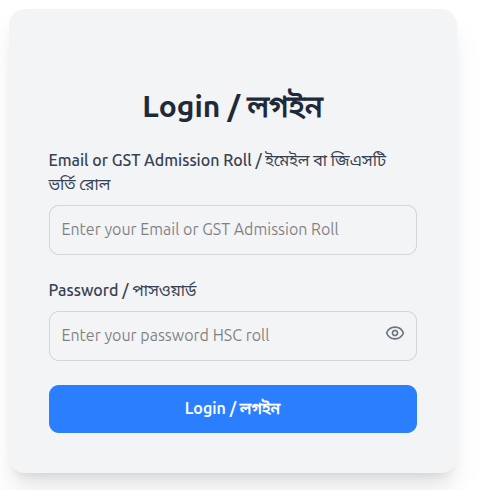
\includegraphics[width=0.6\textwidth]{chapters/chapter4/images/login.png}
    \caption{System Authentication (Login Page)}
    \label{fig:authentication_login}
\end{figure}


\section{Student Module Implementation}
After successful authentication, students are directed to their application portal. The primary task for a student is to complete the comprehensive admission form, providing accurate personal and academic information.

\subsection{Final Admission Form}
The admission form is designed to collect detailed geographical and identification data. To ensure data integrity, the system implements strict front-end validation for each input field.

\begin{figure}[htbp]
    \centering
    % Ensure your file is at this exact path: chapters/chapter4/images/form.png
    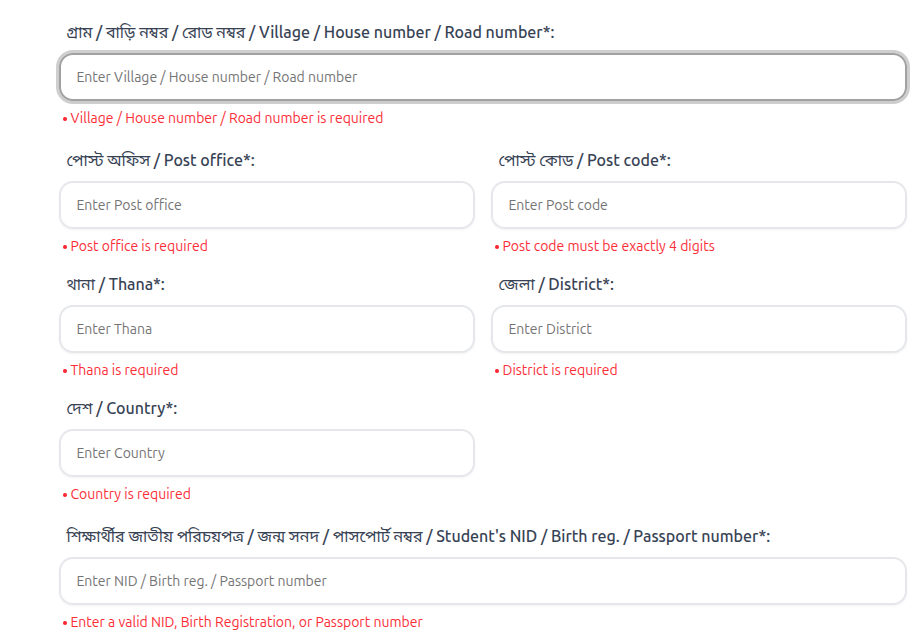
\includegraphics[width=0.85\textwidth]{chapters/chapter4/images/form.png}
    \caption{Student Admission Form with Validation}
    \label{fig:student_form}
\end{figure}

As shown in Figure \ref{fig:student_form}, the form focuses on the following components:

\begin{itemize}
    \item \textbf{Address Details:} The form requires the student's \textit{Village/House number}, \textit{Post Office}, \textit{Thana}, \textit{District}, and \textit{Country}. Each field is marked with an asterisk (*), indicating it is mandatory.
    \item \textbf{Postal Code Validation:} A specific validation rule is applied to the \textbf{Post Code} field, requiring exactly 4 digits, which prevents incorrect data entry.
    \item \textbf{Identification Information:} The system provides a flexible identification section where students must enter either their \textbf{NID}, \textbf{Birth Registration}, or \textbf{Passport number}.
    \item \textbf{Real-time Error Handling:} As illustrated in the figure, the system uses reactive validation. If a user leaves a field empty or enters invalid data (e.g., an incomplete post code), a red error message appears immediately below the input field to guide the user.
    \item \textbf{Bilingual Interface:} Continuing the design philosophy, all labels are provided in both Bengali and English to ensure clarity for all applicants.
\end{itemize}

This structured approach ensures that the database receives clean, formatted data, which simplifies the subsequent verification process by the Dean and Registrar offices.


\subsection{Application Summary and PDF Download}
After completing the necessary steps of the admission form, the student reaches the final stage where they can review their application summary and export the data for official use.

\begin{figure}[htbp]
    \centering
    
\includegraphics[width=0.8\textwidth]{chapters/chapter4/images/download.png}
    \caption{Final Application Submission and Download Interface}
    \label{fig:download_pdf_section}
\end{figure}

The features of this section, as shown in Figure \ref{fig:download_pdf_section}, are described below:

\begin{itemize}
    \item \textbf{Review Mechanism:} The \textit{Previous} button allows students to navigate back and double-check their provided information before final submission. This ensures that no incorrect data is sent to the university database.
    \item \textbf{Instant PDF Generation:} The system is integrated with a PDF generation library that converts the student's input fields into a formal document format. By clicking the \textbf{Download PDF} button, the user can instantly save a copy of their admission form.
    \item \textbf{Visual Feedback:} The button utilizes a distinct gradient color and a download icon to provide clear visual feedback, indicating that this is the primary action of the page.
    \item \textbf{Official Requirement:} This downloaded PDF acts as an acknowledgment slip, which contains a unique identifier for the student. It is mandatory for students to bring a printed copy of this document during the physical verification at the Dean's office.
\end{itemize}
\subsection{Submission Confirmation and Complaint Management}
Once a student successfully submits their application form, the system displays a confirmation message and provides options for subsequent necessary actions. This interface ensures the applicants that their data has been securely stored in the database.

\begin{figure}[htbp]
    \centering
    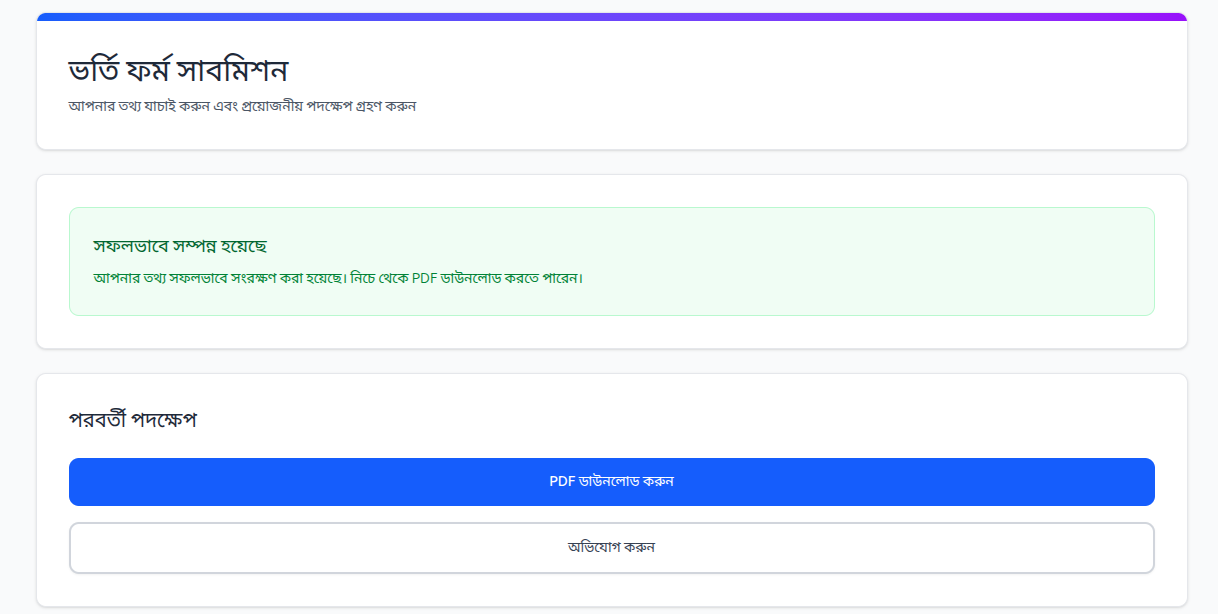
\includegraphics[width=0.85\textwidth]{chapters/chapter4/images/complain.png}
    \caption{Form Submission Confirmation and Complaint Interface}
    \label{fig:submission_status}
\end{figure}

As illustrated in Figure \ref{fig:submission_status}, the submission status page includes several key functional elements:

\begin{itemize}
    \item \textbf{Success Notification:} A green alert box is utilized to inform the student that their information has been successfully saved. This enhances the user experience and maintains system transparency.
    \item \textbf{PDF Generation and Download:} Students can download their completed application form in PDF format for future reference. This is a core component of the system's automated report generation module.
    \item \textbf{Complaint Management:} If a student notices any discrepancy in their data or encounters issues after submission, they can directly file a report through this integrated module.
    \item \textbf{Action Buttons:} The interface features clear and actionable buttons (e.g., "Download PDF" and "Complain"), which guide the user through the next steps without ambiguity.
\end{itemize}

Through this feature, system reliability is increased, and students are provided with immediate feedback and support options.


\section{Admin Module: Data and Resource Management}
The Admin module serves as the primary gateway for preparing the system for a new admission session.

\subsection{Bulk Data Import and External Storage Integration}
The administrator can populate the database by uploading Excel or SQL files containing GST admission results. To ensure data safety, a Google Drive integration is also provided.

\begin{figure}[H]
    \centering
    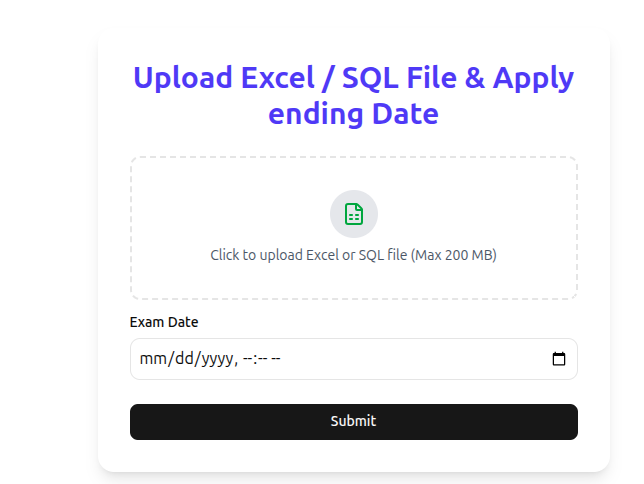
\includegraphics[width=0.75\textwidth]{chapters/chapter4/images/excelupload.png}
    \caption{Excel/SQL File Upload and Application Deadline Interface}
    \label{fig:excel_upload}
\end{figure}

\begin{itemize}
    \item \textbf{Data Ingestion:} The system parses the uploaded file and updates the applicant records. The interface also allows setting an "Exam Date" as a deadline.
    \item \textbf{Cloud Backup:} Using the interface shown in \textit{uploadDrive.png} (if applicable), the admin can sync local data with Google Drive for disaster recovery.
\end{itemize}

\subsection{Examination Announcement}
The admin defines the specific admission unit and the corresponding examination date to notify the applicants.

\begin{figure}[H]
    \centering
    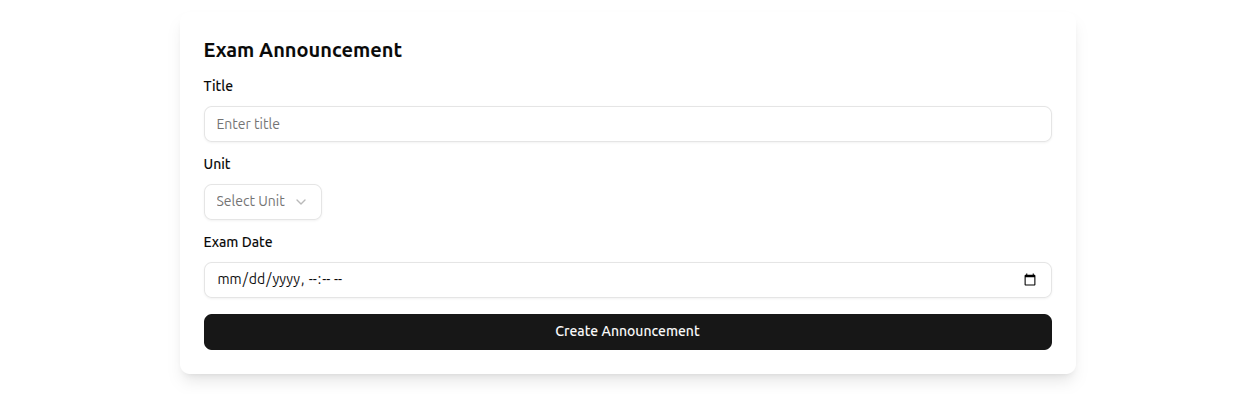
\includegraphics[width=0.75\textwidth]{chapters/chapter4/images/examAnoucement.png}
    \caption{Exam Announcement Configuration Interface}
    \label{fig:exam_announcement}
\end{figure}
\section{Admin Module: User Control and Security}
Security is managed through a comprehensive user administration panel that controls access for university officials.

\subsection{Role-Based Credential Generation}
The Admin can create specific accounts for Deans, Registrars, and Medical Officers using a dedicated credential creation form.

\begin{figure}[H]
    \centering
    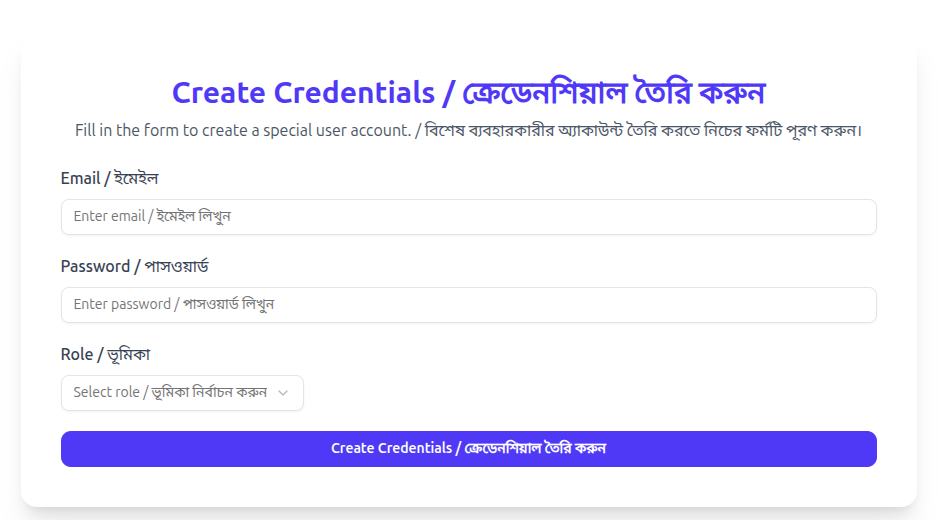
\includegraphics[width=0.75\textwidth]{chapters/chapter4/images/credentail.png}
    \caption{User Credential Creation Interface}
    \label{fig:create_credentials}
\end{figure}

\subsection{System User Monitoring}
A centralized dashboard allows the Admin to monitor all registered officials, their roles, and their account status.

\begin{figure}[H]
    \centering
    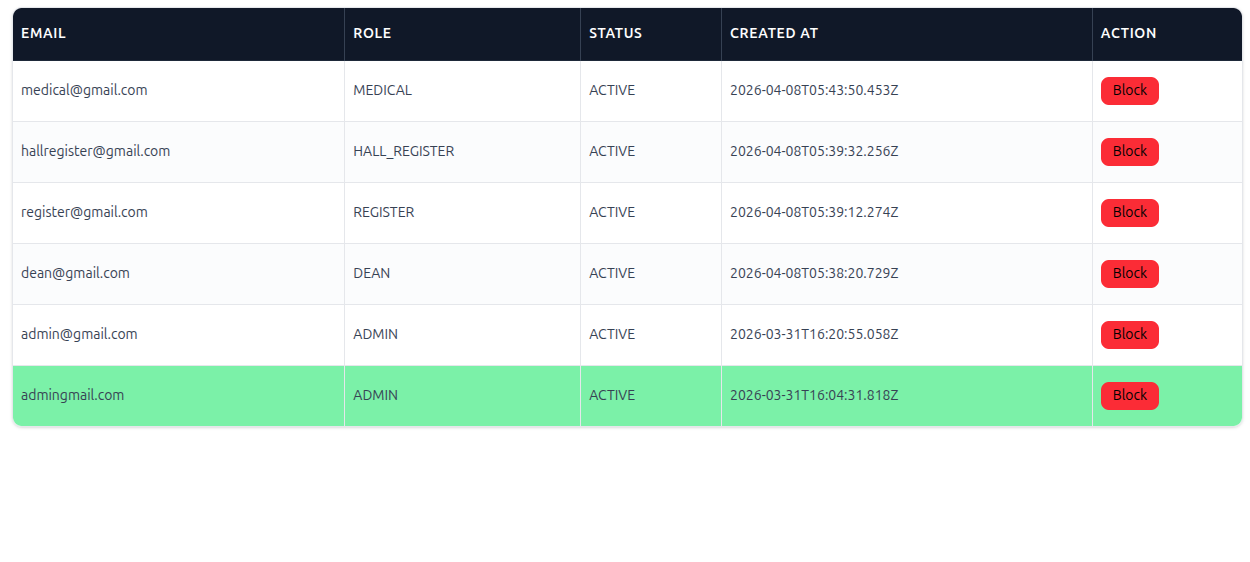
\includegraphics[width=0.9\textwidth]{chapters/chapter4/images/userManagement.png}
    \caption{Administrative User Management Dashboard}
    \label{fig:user_management}
\end{figure}

\begin{itemize}
    \item \textbf{Status Control:} Admins can "Block" or "Unblock" accounts instantly to prevent unauthorized access.
    \item \textbf{Role Identification:} The interface clearly labels the role (e.g., DEAN, REGISTER) and the timestamp of account creation.
\end{itemize}
\section{Admin Module: Complaint Resolution System}
To address student grievances, the Admin panel provides a real-time tracking system for complaints submitted through the student portal.

\subsection{Reviewing Pending Complaints}
All student issues are listed in a simplified queue, allowing administrators to address them systematically.

\begin{figure}[H]
    \centering
    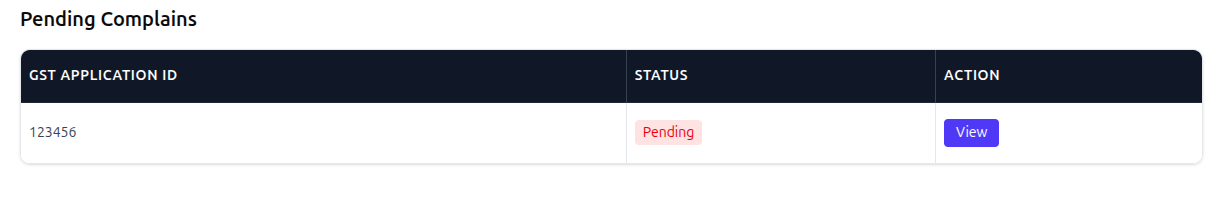
\includegraphics[width=0.85\textwidth]{chapters/chapter4/images/checkcomplain.png}
    \caption{Pending Complaint Tracking Interface}
    \label{fig:check_complain}
\end{figure}

The complaint handling workflow involves:
\begin{itemize}
    \item \textbf{Application ID Mapping:} Every complaint is mapped to a GST Application ID for cross-verifying academic records.
    \item \textbf{Detailed Action:} By clicking the "View" button, the admin can read the full text of the complaint and take necessary corrective measures.
\end{itemize}


% --- Dean Module (Divided) ---
\section{Dean Module: Applicant Verification}
The Dean's primary responsibility is to oversee the departmental applicant lists and verify the academic eligibility of the candidates.

\subsection{Departmental Applicant Queue}
The portal provides a real-time data table displaying students assigned to various departments under the faculty.

\begin{figure}[H]
    \centering
    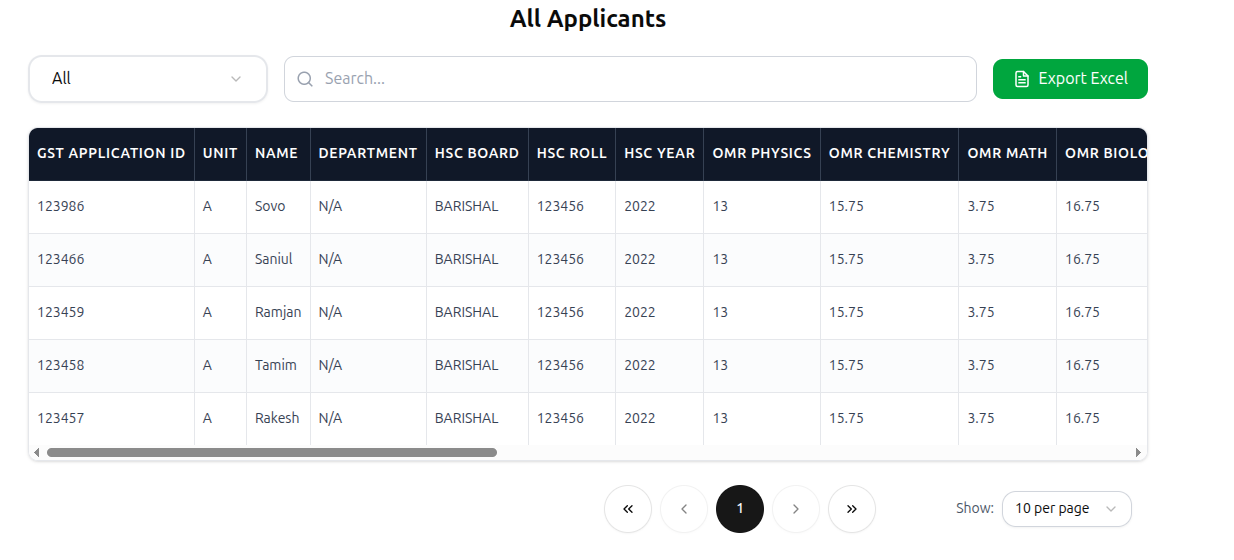
\includegraphics[width=0.9\textwidth]{chapters/chapter4/images/applicantList.png}
    \caption{Dean's Portal: Integrated Applicant List}
    \label{fig:dean_applicant_list}
\end{figure}

\subsection{Detailed Information Table}
To facilitate precise verification, a detailed list table is implemented that shows specific student attributes.

\begin{figure}[H]
    \centering
    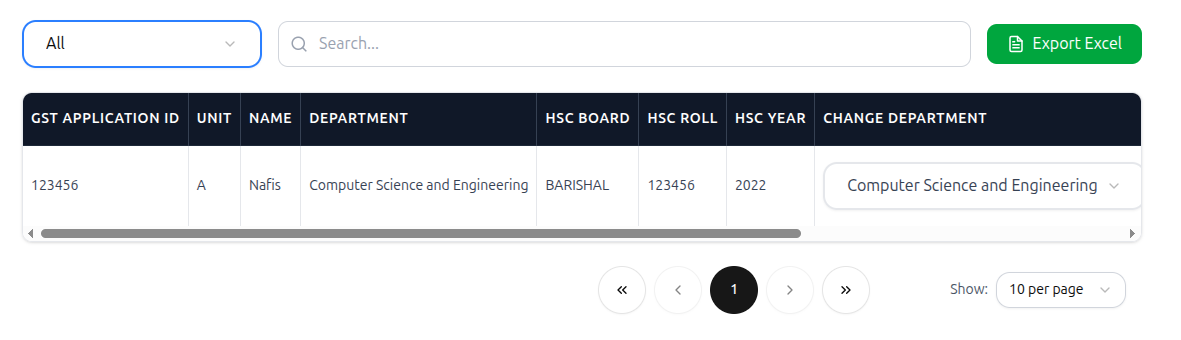
\includegraphics[width=0.9\textwidth]{chapters/chapter4/images/listTable.png}
    \caption{Dean's Detailed Data Verification Table}
    \label{fig:dean_list_table}
\end{figure}

The Dean uses this interface to cross-check GST scores and departmental requirements before moving to the approval stage.
\section{Dean Module: Student Status Management}

\noindent The Dean Module is for managing the status of students. The Dean has the power to approve a student for a department or cancel their application if there are problems with their records.

\setlength{\fboxsep}{6pt}
\setlength{\fboxrule}{1pt}
\begin{figure}[H]
    \centering
   \fbox{ 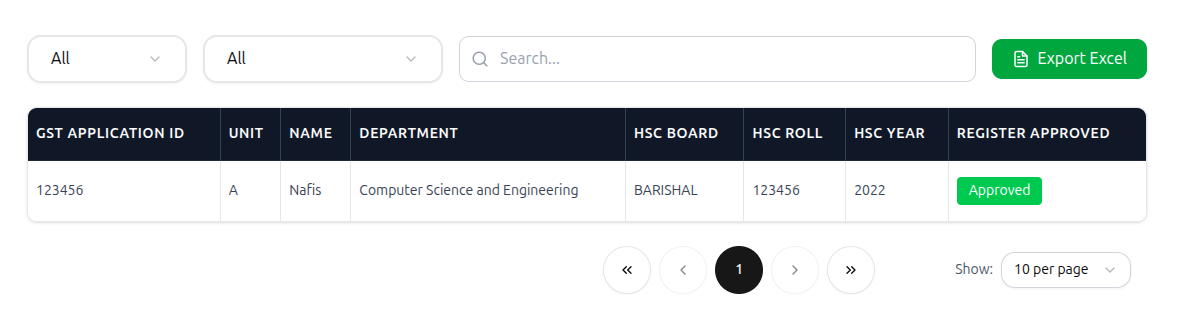
\includegraphics[width=0.8\textwidth]{chapters/chapter4/images/approvedList.png}}
    \caption{Dean’s Portal: Admission Approval and Cancellation Interface}
    \label{fig:dean_status_manage}
\end{figure}

\noindent The Dean can do these things:
\begin{itemize}
    \item {Approve Admission:} If a student's grades and documents are okay, the Dean can click the "Approve" button to send the student to the next step.
    \item {Cancel Admission:} If a student's information is fake or they do not meet the requirements of the department, the Dean can cancel their admission status.
\end{itemize}

\noindent The Dean Module is part of the Student Status Management system. The Dean uses the Deans Portal to make decisions about student admissions. The Dean’s decisions are final and affect the students’ status in the system. The Dean can cancel a student’s admission at any time.
% \section{Dean Module: Data Redundancy and Sync}
To ensure the security of academic records, the Dean's module is equipped with an automated data synchronization feature.

\subsection{Google Drive Integration}
The system allows the Dean to sync the verified applicant lists directly to a faculty-specific Google Drive account.

\begin{figure}[H]
    \centering
    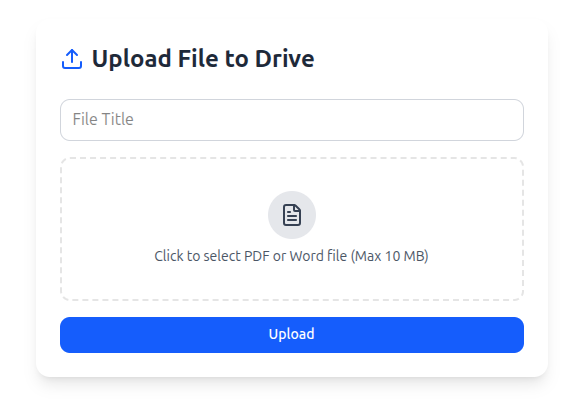
\includegraphics[width=0.7\textwidth]{chapters/chapter4/images/uploadDrive.png}
    \caption{Faculty Data Synchronization with Cloud Storage}
    \label{fig:dean_drive}
\end{figure}

This integration serves as a disaster recovery measure, ensuring that the Dean's office maintains a permanent record of all admitted students even in the event of local server issues.

% --- Registrar Module (Divided) ---
\section{Registrar Module: Centralized Data Validation}
The Registrar office holds the authority for the final validation of applicant data before the admission is officially confirmed. 

\subsection{Master Applicant Queue}
The Registrar monitors the global applicant list to oversee the progress of the admission session across all faculties.

\begin{figure}[H]
    \centering
    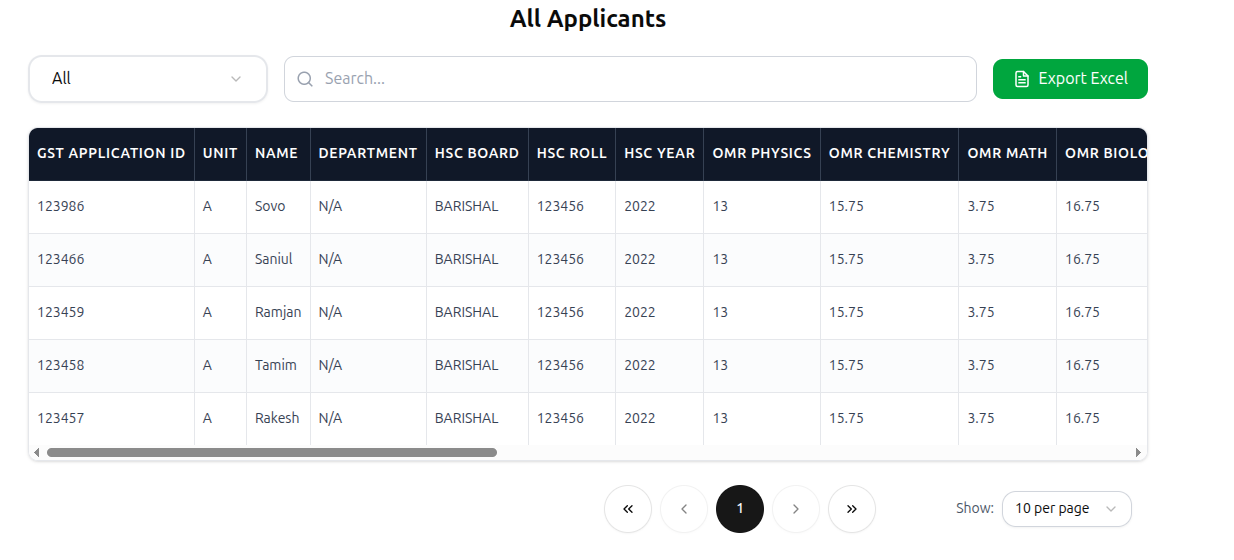
\includegraphics[width=0.9\textwidth]{chapters/chapter4/images/applicantList.png}
    \caption{Registrar's Master Applicant Data Interface}
    \label{fig:registrar_master_list}
\end{figure}

\subsection{Detailed Verification Matrix}
Using a more granular data table, the Registrar office cross-checks the physical document submission status with the digital records.

\begin{figure}[H]
    \centering
    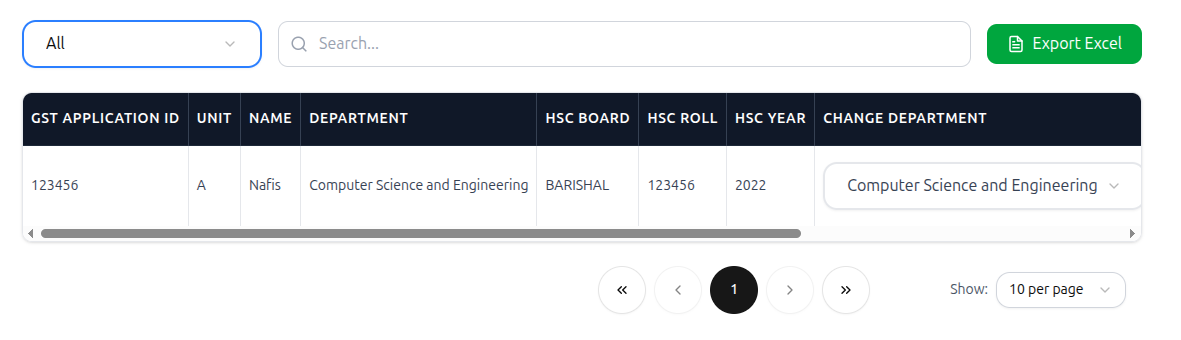
\includegraphics[width=0.9\textwidth]{chapters/chapter4/images/listTable.png}
    \caption{Registrar's Detailed Validation Table}
    \label{fig:registrar_table_view}
\end{figure}

This dual-layer verification ensures that only students with legitimate academic credentials and fee payments are processed for the final step.
\section{Registrar Module: Data Archiving and Redundancy}
As the primary record-keeper of the university, the Registrar's module emphasizes permanent data storage and cloud synchronization.

\subsection{Automated Cloud Backup}
To prevent data loss and ensure long-term accessibility, the system integrates a direct upload feature to the university's central Google Drive.

\begin{figure}[H]
    \centering
    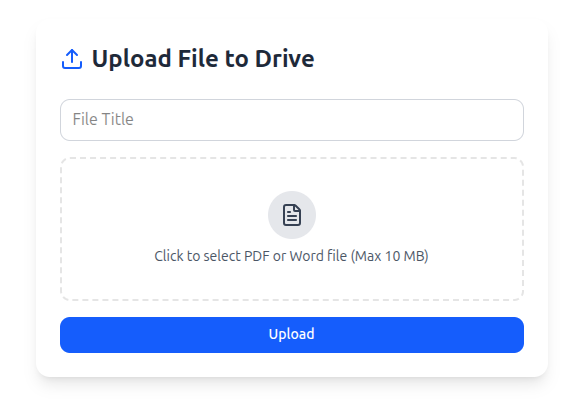
\includegraphics[width=0.7\textwidth]{chapters/chapter4/images/uploadDrive.png}
    \caption{Registrar's Archival System (Google Drive Sync)}
    \label{fig:registrar_archive}
\end{figure}

Through this interface, the Registrar can archive the entire session's data, providing a robust disaster recovery plan for the admission system.
\section{Registrar Module: Final Authorization}
The Registrar performs the final audit. This interface allows the Registrar to finalize the admission or reject it if any legal or official requirement is missing.
\setlength{\fboxsep}{6pt}
\setlength{\fboxrule}{1pt}
\begin{figure}[H]
    \centering
   \fbox{ 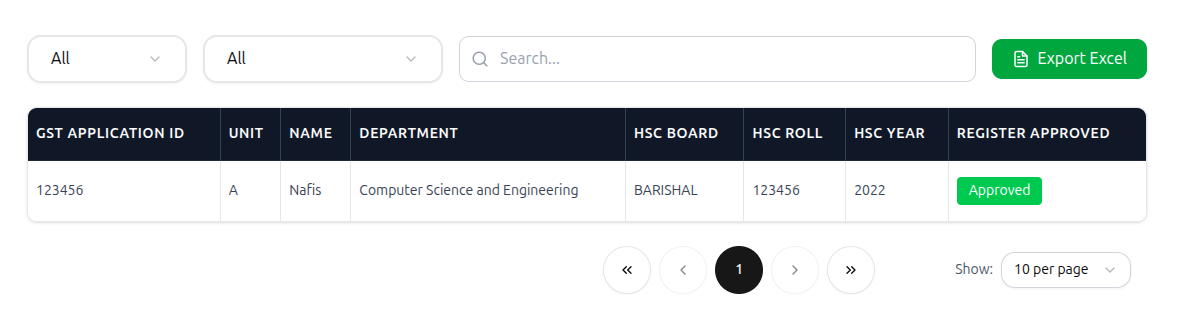
\includegraphics[width=0.8\textwidth]{chapters/chapter4/images/approvedList.png}}
    \caption{Registrar's Final Admission Authorization Dashboard}
    \label{fig:registrar_final_action}
\end{figure}

Through this dashboard, the Registrar ensures:
\begin{itemize}
    \item {Final Confirmation:} Authorized students are officially enrolled in the university database.
    \item {Admission Rejection:} The Registrar can cancel or revert an admission if the payment or official verification fails at the last moment.
\end{itemize}

% --- Hall Registrar Module (Divided) ---
\section{Hall Registrar: Residential Clearance}
The Hall Registrar manages the residential status. Only students with an "Approved" hall status are allowed to reside in the university halls.

\begin{figure}[H]
    \centering
    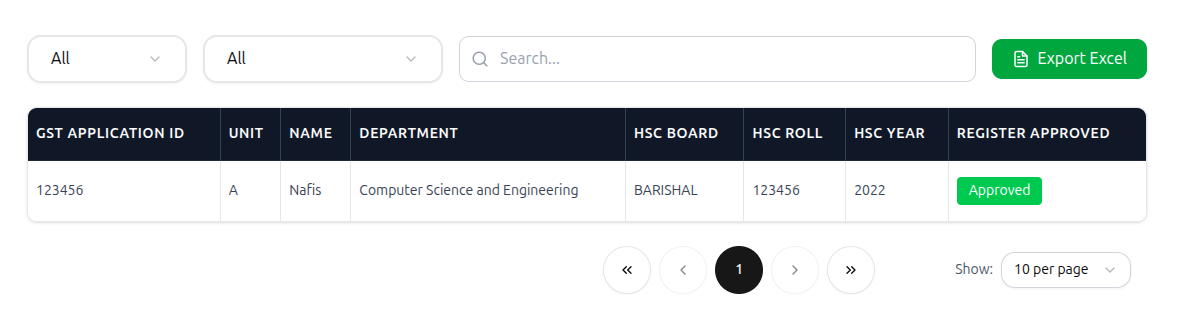
\includegraphics[width=0.85\textwidth]{chapters/chapter4/images/approvedList.png}
    \caption{Hall Allocation Approval and Cancellation View}
    \label{fig:hall_status_manage}
\end{figure}

\begin{itemize}
    \item \textbf{Seat Approval:} Assigning a hall name and room to the student.
    \item \textbf{Allocation Cancellation:} Removing a student from the hall list if they choose to stay off-campus or provide incorrect information.
\end{itemize}
\section{Hall Registrar Module: Resident Data Verification}
To ensure accurate record-keeping, the Hall Registrar utilizes a specialized queue to manage applicants who have applied for residential facilities.

\subsection{Hall Applicant Queue}
The interface displays a list of students who have cleared the academic and administrative stages and are now waiting for residential allocation.

\begin{figure}[H]
    \centering
    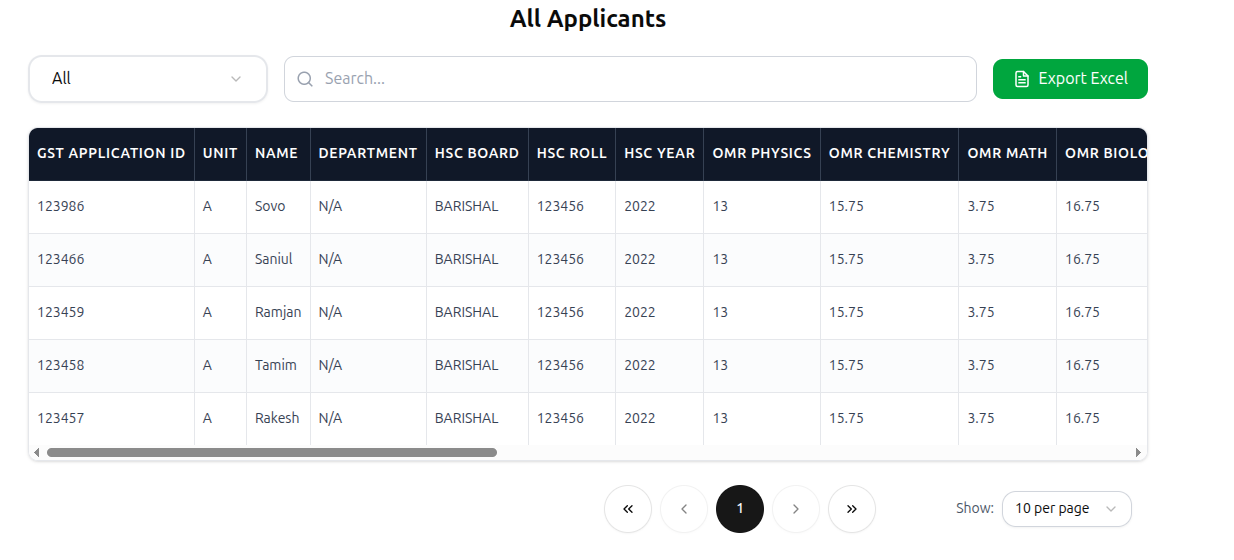
\includegraphics[width=0.9\textwidth]{chapters/chapter4/images/applicantList.png}
    \caption{Hall Resident Applicant Queue}
    \label{fig:hall_applicant_queue}
\end{figure}

\subsection{Detailed Resident Attributes}
The Hall Registrar can view specific student data, such as permanent address and gender, which are crucial factors in hall assignment.

\begin{figure}[H]
    \centering
    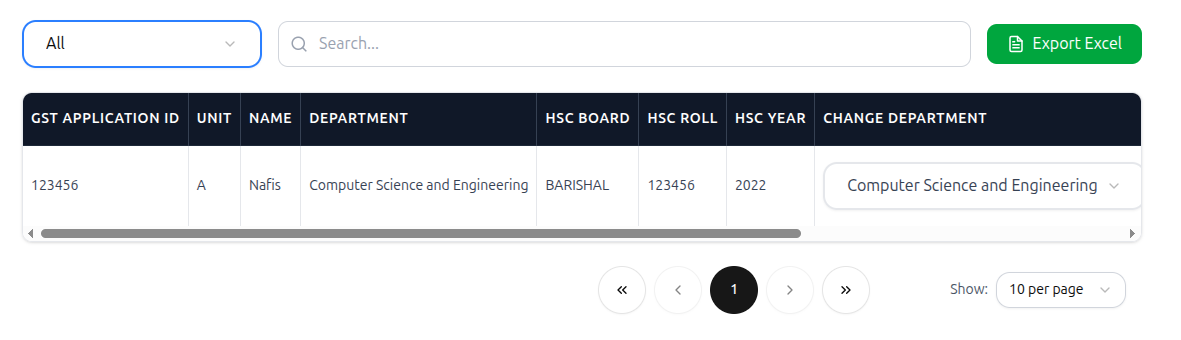
\includegraphics[width=0.9\textwidth]{chapters/chapter4/images/listTable.png}
    \caption{Detailed Resident Information Matrix}
    \label{fig:hall_resident_table}
\end{figure}
\section{Hall Registrar Module: Data Redundancy}
Due to the sensitivity of residential records, the Hall Registrar module includes a dedicated synchronization mechanism to preserve allocation data.

\subsection{Cloud Synchronization for Hall Records}
The Hall Registrar can sync the final residential allotment lists to a secure cloud platform, ensuring that hall offices have access to student data for room distribution.

\begin{figure}[H]
    \centering
    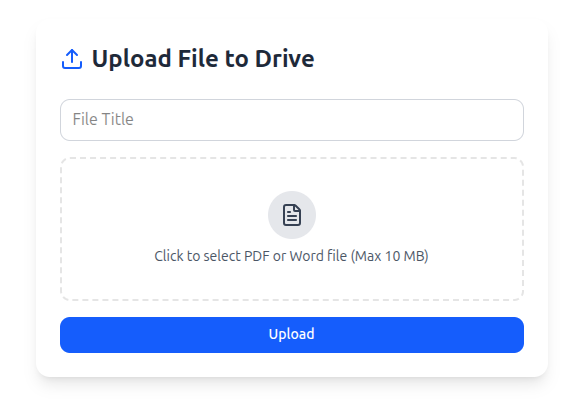
\includegraphics[width=0.7\textwidth]{chapters/chapter4/images/uploadDrive.png}
    \caption{Hall Office Data Sync and Backup}
    \label{fig:hall_drive_sync}
\end{figure}

This feature ensures data integrity and provides an offline reference for hall administration personnel.


% --- Medical Officer Module (Divided) ---
\section{Hall Registrar: Residential Clearance}
The Hall Registrar manages the residential status. Only students with an "Approved" hall status are allowed to reside in the university halls.


\setlength{\fboxsep}{6pt}
\setlength{\fboxrule}{1pt}
\begin{figure}[H]
    \centering
   \fbox{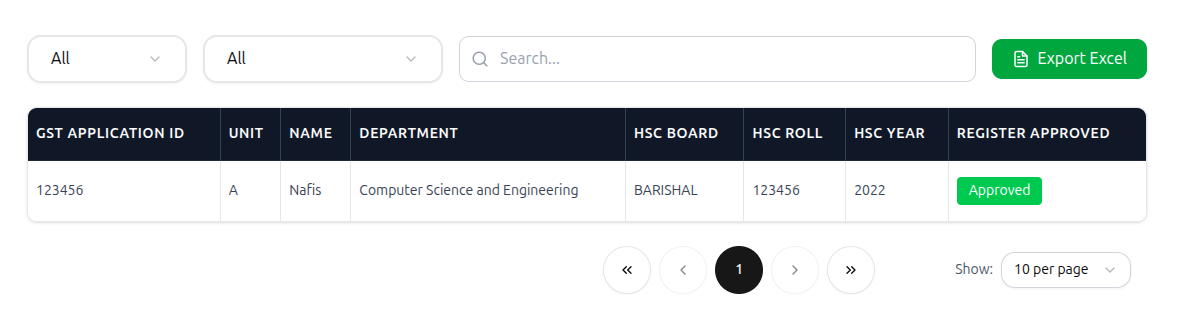
\includegraphics[width=0.8\textwidth]{chapters/chapter4/images/approvedList.png}}
    \caption{Hall Allocation Approval and Cancellation View}
    \label{fig:hall_status_manage}
\end{figure}

\begin{itemize}
    \item {Seat Approval:} Assigning a hall name and room to the student.
    \item {Allocation Cancellation:} Removing a student from the hall list if they choose to stay off-campus or provide incorrect information.
\end{itemize}
\section{Medical Officer Module: Applicant Health Data}
This section allows the Medical Officer to access the list of applicants who are awaiting medical checkups or record verification.

\subsection{Medical Verification Queue}
The portal displays a prioritized list of students who have completed their initial academic formalities and are now eligible for medical screening.

\begin{figure}[H]
    \centering
    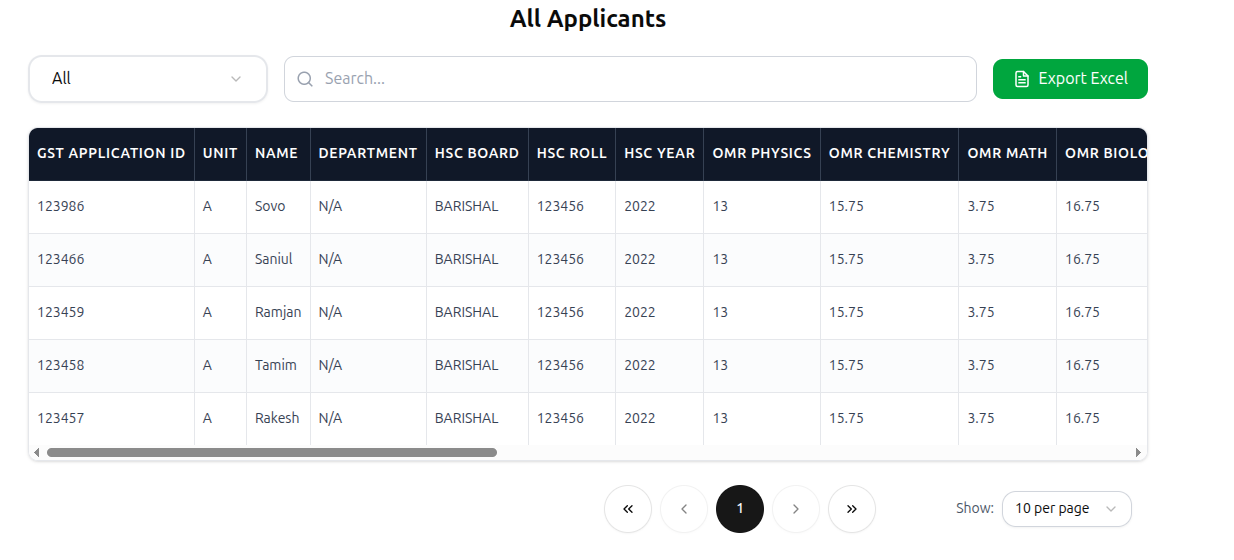
\includegraphics[width=0.9\textwidth]{chapters/chapter4/images/applicantList.png}
    \caption{Medical Officer's Applicant Screening Queue}
    \label{fig:medical_queue}
\end{figure}

\subsection{Detailed Medical Record Matrix}
A specialized table is used to view detailed student attributes, helping the medical staff to identify and document any specific health conditions.

\begin{figure}[H]
    \centering
    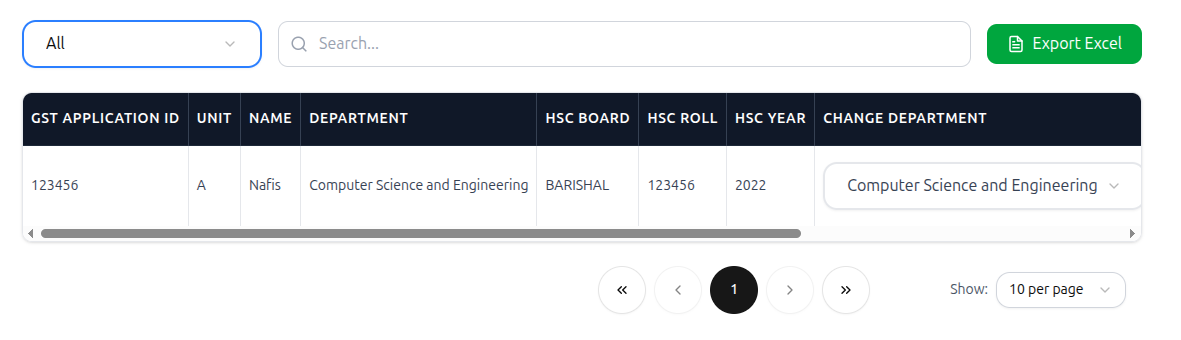
\includegraphics[width=0.9\textwidth]{chapters/chapter4/images/listTable.png}
    \caption{Detailed Health Record and Information Matrix}
    \label{fig:medical_record_table}
\end{figure}
% \section{Medical Officer Module: Data Synchronization}
To ensure the long-term safety of student health records, a cloud synchronization feature is integrated into the Medical Module.

\subsection{Cloud Backup for Health Records}
The Medical Officer can sync all health-related data and clearance reports to the university's central Google Drive for future medical history tracking.

\begin{figure}[H]
    \centering
    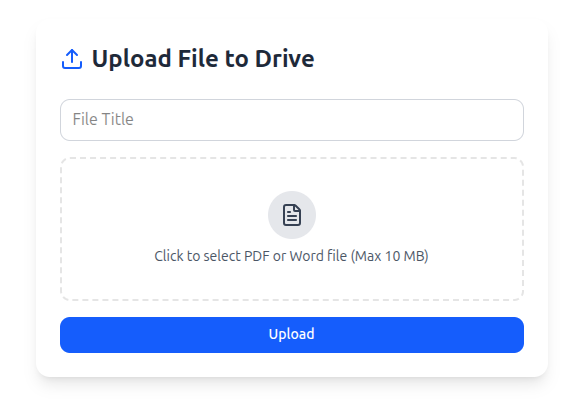
\includegraphics[width=0.7\textwidth]{chapters/chapter4/images/uploadDrive.png}
    \caption{Medical Data Archiving and Drive Integration}
    \label{fig:medical_drive_sync}
\end{figure}

This integration ensures that the university medical center maintains a persistent and secure digital record of all admitted students.